\documentclass{elsarticle}
\biboptions{sort&compress}
\bibliographystyle{alpha}



\usepackage{amssymb}
%\setcounter{tocdepth}{3}
\usepackage{graphicx} 

% HASKELL SYNTAX HIGHLIGHTING - MUST BE LOADED BEFORE xcolor and listings IF THEY'RE ALSO BEING USED
\usepackage{mpshaskell}
\newcommand{\code}[1]{\haskell{#1}}
\newCodeWord{tree,list,original,reversed,x,xs,f,f',f'',y,ys,tour_x,tour_y,ex,ey,h,h',h'',e,e1,e2}
\newFunction{empty,singleton,member,reroot,splice,error,select,link,fromList',cut,path,guard,father}
\newSymbol{\insertL}{\lhd}
\newSymbol{\insertR}{\rhd}
% END OF HASKELL SYNTAX HIGHLIGHTING

% ADDED BY MIKE
\newcommand{\madd}[1]{\textcolor{Purple}{#1}}
\newcommand{\mdel}[1]{\textcolor{Yellow}{#1}}

\usepackage{xspace}
\newcommand{\MATHSF}[1]{\ensuremath{\mathsf{#1}}\xspace}
\newcommand{\link}{\MATHSF{link}}
\newcommand{\cut}{\MATHSF{cut}}
\renewcommand{\root}{\MATHSF{root}}
\newcommand{\reroot}{\MATHSF{reroot}}
\newcommand{\connected}{\MATHSF{connected}}
% END OF MIKE'S ADDITIONS


\usepackage{xcolor}

\usepackage{url}
%\urldef{\mailjm}\path|{jcsaenzcarrasco1, m.stannett}@sheffield.ac.uk|    
\newcommand{\keywords}[1]{\par\addvspace\baselineskip
\noindent\keywordname\enspace\ignorespaces#1}

\newcommand{\tcr} [1]{\textcolor{red}{#1}}
\newcommand{\tcb} [1]{\emph{\textcolor{blue}{#1}}}


\begin{document}
\title{Dynamic Trees through Euler Tours\\%
\large{A purely functional programming approach}}

\author{J.C.~Saenz-Carrasco\fnref{conacyt}\corref{cor1}}
\ead{jcsaenzcarrasco1@sheffield.ac.uk}

\author{M.~Stannett}
\ead{m.stannett@sheffield.ac.uk}

\address{Department of Computer Science,\\
Regent Court, 211 Portobello,\\
Sheffield S1 4DP, United Kingdom}

\cortext[cor1]{Corresponding author}
\fntext[conacyt]{Postgraduate research student, supported by the Consejo Nacional de Ciencia y Tecnolog\'{i}a, CONACYT (Mexican National Council for Science and Technology) under grant 411550, scholar 580617, CVU 214885.}

\begin{abstract}
We present purely-functional data structures for managing dynamic updates and queries, by combining the structure of Hinze and Paterson's finger tree with an efficient binary search tree to handle Euler tours as sequences: like its imperative counterpart, our proposal supports $O(\log n)$ amortised complexity per operation, where $n$ is the number of the vertices in the tree. While existing data structures mirror these time bounds, ours is arguably the first to provide all three of the basic dynamic tree operations (\link, \cut and \connected) within a single functional structure. To illustrate how the algorithms perform in practice we have implemented them in Haskell and conducted various benchmarking experiments. The data support our claims, while also pointing to remaining inefficiencies. We discuss these in detail and suggest possible ways forward.
\end{abstract}

\begin{keyword}
Dynamic tree algorithms \sep functional programming \sep persistent data structures \sep Haskell
\end{keyword}


\maketitle




\section{Introduction}
\label{sec:Intro}

In this paper we show how functional programming features (for example, the use of lazy evaluation) can be exploited in the context of modelling massive dynamically changing networks. Such networks are increasingly ubiquitous and provide important value-added to modern commerce and society. With growing size, however, comes additional computational overheads, and it is important to identify low-complexity, preferably sub-linear, algorithms for such heavily utilised tasks as path-finding, re-routing and dynamic workload distribution.

Our contribution in this paper is to provide a novel functional programming data structure for network representation that allows the programming of suitable low-complexity algorithms, and we provide experimental confirmation of our performance claims. As explained in more detao; below, we work with collections of spanning trees (one for each connected component of the network), and in this context our operations show the following complexities (Figure)

\begin{center}
\begin{table}
\begin{tabular}{||l | l | c||} 
\hline
Function & Description & Complexity \\ %[0.5ex] 
\hline\hline
\texttt{linkTree} 
  & 
  & $O(m\log n)$ \\
\texttt{cutTree} 
  &
  & $O(\log n)$ \\
\hline
\texttt{conn} 
  & 
  & $O(\log n)$ \\ 
\texttt{link} 
  & 
  & $O(m\log n)$ \\
\texttt{cut} 
  & 
  & $O(\log n)$ \\
\hline
\texttt{reroot} 
  &  
  & $O(\log n)$ \\
\texttt{root} 
  & 
  & $O(1)$ \\
\hline   
\end{tabular}
\caption{Amortised time complexity for various dynamic network-editing operations in terms of their effect on the associated forest of spanning trees. In each case, $n$ gives the number of vertices in the first (or only) tree operated upon; for those functions taking two trees as input, $m$ i the number of vertices in the second tree. The result for \link assumes that $m \leq n$ (if not, we can swap the order of the arguments before applying the algorithm).}
\end{table}\end{center}



give first work-optimal bounds for managing dynamic trees for purely functional data structures. We do this not only for extending the application of finger trees, we offer a solution for dynamic connectivity when facing persistent data structures as well as providing a simple interface to the user. The \dyntset exposes two types, \texttt{Tree} and \texttt{Forest}, to the user. The following is a compilation of \tcb{OUR} the functions, types and times we have implemented in Haskell, on top of that done by Hinze and Paterson \cite{FTs}:

\begin{center}
\small
 \begin{tabular}{||l | l | c||} 
 \hline
 Function & Type & Time complexity \\ %[0.5ex] 
 \hline\hline
 \texttt{linkTree} & \texttt{Vertex} $\to$ \texttt{Tree} $\to$ \texttt{Vertex} $\to$ \texttt{Tree} $\to$ \texttt{Tree} & $O(m\log n)$ \\
 \texttt{cutTree} & \texttt{Vertex} $\to$ \texttt{Vertex} $\to$ \texttt{Tree} $\to$ \texttt{(Tree,Tree)} & $O(\log n)$ \\
 \hline
 \texttt{conn} & \texttt{Vertex} $\to$ \texttt{Vertex} $\to$ \texttt{Forest} $\to$ \texttt{Bool} & $O(\log n)$ \\ 
 \texttt{link} & \texttt{Vertex} $\to$ \texttt{Vertex} $\to$ \texttt{Forest} $\to$ \texttt{Forest} & $O(m\log n)$ \\
 \texttt{cut} & \texttt{Vertex} $\to$ \texttt{Vertex} $\to$ \texttt{Forest} $\to$ \texttt{Forest} & $O(\log n)$ \\
 \hline
 \texttt{reroot} & \texttt{Tree} $\to$ \texttt{Vertex} $\to$ \texttt{Tree} & $O(\log n)$ \\
 \texttt{root} & \texttt{Tree} $\to$ \texttt{Maybe(Vertex)} & $O(1)$ \\
 \hline   
\end{tabular}
where $n$ and $m$ are the corresponding sizes of the trees involved; when $linking$ is performed, then the constraint $m \leq n$ should taken into account
\end{center}
\normalsize 


In general, the number of vertices in such a network can change from one moment to the next, and as new edges are introduced and existing one deleted, the underlying topology of the network will change, with connected components merging and separating as time passes. The problem we address is one of the simplest we can ask about a network, but at the same time one of the most fundamental, namely: \emph{given two vertices, $u$ and $v$, do they belong to the same component}? The answer, of course, will depend on when we ask the question, because the system we're considering is \emph{dynamic}; new connections can be created between vertices and old ones can be deleted.

If we are to answer this question efficiently, it follows that we need to use a dynamic data type to store information about the network, its vertices, and edges. Our goal is to ensure that updates to the network will result in only local changes to the data representation; we do not want to recompute the entire representation simply because one edge has been added or removed. Our approach is first to represent connected components not as graphs but as spanning trees, and then to use a novel approach to representing these trees dyanmically. [discussion: While adding a vertex to a component and adding it to the spanning tree are equivalent tasks, breaking an edge in the spanning tree corresponds to breaking multiple edges in the underlying component.]



Given our use of spanning trees to represent connected components, this question becomes: \emph{do $u$ and $v$ belong to the same tree}? Notice that adding new links within an already connected component does not affect its existing spanning trees; although new spanning trees may become possible, no existing spanning tree loses that status. On the other hand, if we connect vertices from distinct components, joining those nodes in the associated spanning trees automatically creates a new spanning tree for the larger component created by adding the link. (The relationship between deleting an edge in a component vs. deleting it in its spanning tree is more complex--see Sect.~\ref{sec:discussion}.)  We accordingly assume that the forest can change dynamically in response to repeated applications of two basic operations: \link and \cut. 
\begin{itemize}
\item
  if vertices $u$ and $v$ belong to different trees, $\link(u,v)$ adds the edge $(u,v)$ to the forest, thereby causing the trees containing $u$ and $v$ to be joined together to form a new, larger, tree; if the vertices already belong to the same tree, the operation has no effect. Formulated in this way, the function \link, can be denoted as
\item
  if vertices $u$ and $v$ are connected by an edge, $\cut(u,v)$ removes that edge, thereby causing the tree that contains it to be split into two smaller trees; if the vertices are not connected, the operation has no effect. 
\end{itemize}

\madd{WORKING HERE}

The problem has been studied as \textit{dynamic trees} under different variants according to the application, for instance, Sleator and Tarjan defined the \textit{link-cut} tree for solving network flow problems \cite{DS-DynTs}, Henzinger and King provided \textit{Euler tour} (ET) trees for speeding up dynamic connectivity on graphs \cite{Rand-DynGs-Algos} or Frederickson describing the \textit{topology} tree for maintaining the minimum spanning tree \cite{DSs-Online-Upd-MSTs}. The former and latter trees are based on techniques called \textit{path-decomposition} and \textit{tree contraction} respectively. In this paper we are interested on Euler tour trees, a technique called \textit{linearisation}, since the original tree (of any degree) is flattened and handled it as a sequence, in other words, turning a non-linear structure into a linear one.

All the above techniques have been implemented and studied for ephemeral data structures, performing $O(\log n)$ per operation. Functional data structures, on the other hand, ease the reasoning and implementation for the cases when preserving history is needed as in self-adjusting computation \cite{DynamizingAlgos} or as in version control \cite{CVS-Demaine}. To overcome the lack of pointers, researchers have devised data structures to represent efficient sequences, most notably, \textit{finger trees} \cite{FTs}. This structure performs well, allowing updates and queries in logarithmic time. We introduce the \emph{dynamic trees through Euler-tours}, a variant of the Hinze's and Paterson finger trees, or \dyntset for short. Like the finger tree, the \dyntset edit sequences in logarithmic time while providing dynamic tree operations. The key insight is to make $O(1)$ steps to perform \textit{connected}, \textit{link}, and \textit{cut} in logarithmic time. In Section \ref{sec:TechDes} we show this for \textit{connected} and \textit{cut}, whereas \textit{link} takes $O(m \log n)$. In Section \ref{sec:Eval} we show that, in practice, different results can be obtained, such $O(1)$ per operation as long as \link is interleaved with \cut.
 \tcb{NO FURTHER explanation about the $O(1)$ performance}

\madd{MOVED THIS TO TOP -- NEEDS A BIT IF REWRITING}

The contribution of this paper is to give first work-optimal bounds for managing dynamic trees for purely functional data structures. We do this not only for extending the application of finger trees, we offer a solution for dynamic connectivity when facing persistent data structures as well as providing a simple interface to the user. The \dyntset exposes two types, \texttt{Tree} and \texttt{Forest}, to the user. The following is a compilation of \tcb{OUR} the functions, types and times we have implemented in Haskell, on top of that done by Hinze and Paterson \cite{FTs}:

\begin{center}
\small
 \begin{tabular}{||l | l | c||} 
 \hline
 Function & Type & Time complexity \\ %[0.5ex] 
 \hline\hline
 \texttt{linkTree} & \texttt{Vertex} $\to$ \texttt{Tree} $\to$ \texttt{Vertex} $\to$ \texttt{Tree} $\to$ \texttt{Tree} & $O(m\log n)$ \\
 \texttt{cutTree} & \texttt{Vertex} $\to$ \texttt{Vertex} $\to$ \texttt{Tree} $\to$ \texttt{(Tree,Tree)} & $O(\log n)$ \\
 \hline
 \texttt{conn} & \texttt{Vertex} $\to$ \texttt{Vertex} $\to$ \texttt{Forest} $\to$ \texttt{Bool} & $O(\log n)$ \\ 
 \texttt{link} & \texttt{Vertex} $\to$ \texttt{Vertex} $\to$ \texttt{Forest} $\to$ \texttt{Forest} & $O(m\log n)$ \\
 \texttt{cut} & \texttt{Vertex} $\to$ \texttt{Vertex} $\to$ \texttt{Forest} $\to$ \texttt{Forest} & $O(\log n)$ \\
 \hline
 \texttt{reroot} & \texttt{Tree} $\to$ \texttt{Vertex} $\to$ \texttt{Tree} & $O(\log n)$ \\
 \texttt{root} & \texttt{Tree} $\to$ \texttt{Maybe(Vertex)} & $O(1)$ \\
 \hline   
\end{tabular}
where $n$ and $m$ are the corresponding sizes of the trees involved; when $linking$ is performed, then the constraint $m \leq n$ should taken into account
\end{center}
\normalsize 

The first block (first two rows) contains the functions to perform dynamic tree operations. The following block (rows 4, 5 and 6) lists the functions that compute an unbounded, although finite, sequence of dynamic tree operations over the same forest $F$. Finally, last two rows are the core functions, apart from the ones provided by Hinze and Paterson work \cite{FTs}. 
%, to perform dynamic tree operations. \tcb{PERHAPS explain the above table widely or paraphrasing ???}

In the next section, we give an overview of the finger tree functions and their performance. These are the foundations for our functions altogether with some of the functions from the Hackage library \texttt{Data.Set} \footnote{https://hackage.haskell.org/package/containers-0.5.10.2/docs/Data-Set.html} which mimic the set-like operations over our functions, such as testing membership. 

%In Section~\ref{sec:Example}, we present an in-depth example using the operations mentioned above. In particular, we depict how the \dyntset manages the trees as sequences under the dynamic setting, showing how the \dyntset structure is constructed immutably. 
In Section \ref{sec:TechDes}, we describe our implementation for performing dynamic tree operations with purely data structures, the \dyntset. The following is the address where our source code is hosted and publicly available:
\begin{center}
\url{https://github.com/jcsaenzcarrasco/ETdynTs}
\end{center}

We evaluate \dyntset empirically in Section~\ref{sec:Eval}. In concrete, we plot the results of benchmarking the functions in the first two sections of the table above. Our evaluation demonstrates that \dyntset performs according the function definitions with a constant factor between \conn and \link and \cut. 

%Section~\ref{sec:Discuss} discuss the main reasons we took into account when designing ETFT, with some suggestions for improving the internal vertex annotations. 
In Section~\ref{sec:RelWrk} we suggest potential alternatives for designing dynamic data structures to solve the problem described in the present document. 

Finally, we conclude in Section~\ref{sec:Concl} with a summary of our work.


\tcr{Presentationally I'm missing a better description of the background material. The paper recalls the definition of a monoid, but does not recall the definition of an Euler tour nor give enough detail on finger trees to read as an independent document.} 




\tcr{---------- P O S I T I V E    C O M M E N T S ------------------}


\tcr{This paper introduces Euler Tour Finger Trees (ETFTs), a persistent, purely-functional tree and forest data structure that supports O(log n) complexity for all operations, including link and cut. It gives an implementation in Haskell.}

\tcr{At a high-level, the tree is represented as an Euler Tour (a list of vertex pairs describing a path through the tree), which in turn is represented by a finger tree, thereby allowing O(log n) concatenation and splitting. That allows manipulating Euler tours efficiently, and building interesting tree operations easily.}

\tcr{Most of the implementation in this paper thus builds on existing implementations of finger trees and sets. Yet the combination seems novel, and the complexity bounds of the ETFT operations follow almost trivially, which is nice.
The paper presents a functional data structure for maintaining a dynamic forest under link and cut operations. It realizes this in O(log n) time complexity per operation (amortized), using an Euler tour tree representation implemented using a combination of finger trees and sets. }

\tcr{The paper first recalls dynamic trees and their operations, and then monoids, sets implemented with balanced search trees, Euler-tour trees and finger trees. It then gives (graphical) examples of how the sets and finger trees fit together to realize dynamic trees, it recalls graphically the root, reroot, split, concatenation, and view operations of finger trees, and then walks through the implementation of root, reroot, connected, link, and cut.
Finally the paper contains experiments illustrating that the implementation meets the claimed complexity bounds and discusses related and future work.
This is an interesting piece of work.}
%\end{comment}


\section{Preliminaries} 
\label{sec:Prelim} 

Our work and contribution relies mainly on three structures, a \textit{monoid}, a \textit{set} and a \textit{finger tree}, which are briefly described in the following subsections. 

\subsection{Monoid}

A \textit{monoid} is a triple $(S,\star,e)$, where $S$ is a set, $\star$ is a binary operation, called $product$ and $e$ is an element of $S$, called $unit$, satisfying the following properties:

\begin{enumerate}
\item $e \star x = x = x \star e$, for all $x \in S$ 
\item $x \star (y \star z) = (x \star y) \star z $, for all $x,y,z \in S$.  
\end{enumerate}

As an example of a Haskell implementation of a monoid we have:
%\begin{verbatim}
\begin{lstlisting}[mathescape]
class Monoid  a where 
   mempty  :: a
   mappend :: a $\to$ a $\to$ a
\end{lstlisting}   
%\end{verbatim}

where the function \code{mempty} represents the element $e$ and the function \code{mappend} represents function $\star$. Detailed information about monoids within the functional programming can be found in \cite{Monoids}, and for the Haskell implementation at \cite{HaskellMonoid}.


\subsection{Set as binary search tree}
A \textit{binary search} tree (BST) is either a \textit{leaf} (also called a \code{tip}) or a vertex consisting of a \textit{value}, a \textit{left} BST and a \textit{right} BST. The height of the tree determines the time taken to perform every operation onto it, therefore the shorter the height the better, and this is done throughout a \textit{balancing scheme}. The study of BSTs is vast and there are several implementation around. In our case, a \textit{size balanced} is used. A detailed comparison and benchmarking is outside the scope of the present work.

\tcr{My main criticism of the paper is the presentation. While I appreciate the use of diagrams in the first half of the paper, high-level explanations are missing later. The paper does not do a very good job providing an intuition for how the data structure works. For example, I was struggling understanding the role of the monoidal set. The paper also explains too little of the background regarding used existing data structures and their realisation in Haskell libraries. For example, the interface to the finger tree ADT and the Measured type class. In general, most of the explanations are closely tight to the code but don’t give a high-level picture of what individual operations do in terms of the Euler tour. Given that there is plenty of space left in the paper, this could be improved in the final version.}


The following is an snippet of \code{Data.Set} \footnote{https://hackage.haskell.org/package/containers-0.5.10.2/docs/Data-Set.html}
%\begin{verbatim}
\begin{lstlisting}
data Set a    = Bin Size a (Set a) (Set a)
              | Tip
\end{lstlisting}              
%\end{verbatim}

In Table~\ref{tab:Setfuncs} we show the set-functions we have incorporated in ETFT from \code{Data.Set}.
\small
\begin{table}
\begin{center}
\begin{tabular}{||l | l | c||} 
 \hline
 Function         & Type                                   & Time complexity            \\ 
 \hline\hline
 \texttt{empty}   & \texttt{Set a}                         & $O(1)$                     \\ 
 \hline
 \texttt{insert}  & \texttt{a $\to$ Set a $\to$ Set a}     & $O(\log n)$                \\
 \hline
 \texttt{member}  & \texttt{a $\to$ Set a $\to$ Bool}      & $O(\log n)$                \\ 
 \hline
 \texttt{union}   & \texttt{Set a $\to$ Set a $\to$ Set a} & $O(m(\log\frac{n}{m} +1))$ \\
 \hline
\end{tabular}
\caption{Leijen's implementation of \code{Data.Set} \cite{HaskellSet}, based on \cite{ParallelSets}}
\label{tab:Setfuncs} 
\end{center}
\end{table}
\normalsize

Functions \code{empty} and \code{union} are, in fact, the monoidal functions \code{mempty} and \code{mappend} respectively. 

\subsection{Euler-tour tree} 

Dealing with trees of different degree can be complicated. A simpler way to handle and represent trees of any degree is by an Euler tour. To represent a tree $t$, we replace every edge $\langle u,v \rangle$ of $t$ by two arcs $(u,v)$ and $(v,u)$, and add a loop $(v,v)$ to represent each vertex $v$. In this context, a tree $t$ can have at least one, and in general, many Euler tours. The size of an Euler tour \textit{et} of $t$ is $et(t) = 2v + 2e - 1$, where $v$ is the number of vertices of $t$ and $e$ its number of edges. We can represent an Euler tour in Haskell simply as a list of pairs, such in 

%\begin{verbatim}
\begin{lstlisting}
data EulerTour a = [(a,a)] 
\end{lstlisting}
%\end{verbatim}

We will see that represent tours in this way is efficient since they will be managed by the finger tree with performance explain shortly and in Section~\ref{sec:TechDes}. 

\subsection{Finger tree} 

We present Hinze and Paterson's non-strict version of finger trees \madd{(FTs)} \cite{FTs}, followed by the functions we have used for the ETFT.
%\begin{verbatim}
\begin{lstlisting}
data FingerTree v a = Empty
                    | Single a 
                    | Deep v 
                           Digit a 
                           FingerTree v (Node v a) 
                           Digit a
\end{lstlisting}                           
%\end{verbatim}


\tcr{This reviewer can't help but think that there seems to be a lot of redundancy in the proposed data structure, as the Euler tour node pairs are present in both the sets and in the finger trees.}


\code{Digit} type holds from one up to four elements of type \code{a}. \code{Node} type can hold two or three elements of type \code{a}. The recursive and nested definition of \code{FingerTree} forces the structure to be balanced by the types, instead of enforced it by code invariants. Finger trees are 2-3 trees where values are stored at the leaves, in our case an Euler tour formed by pairs of those values. To implement \textit{search}, \textit{insert} and \textit{lookup} efficiently, Hinze and Paterson \cite{FTs} added a monoidal annotation on the intermediate vertices, the \code {v} type.

\small
\begin{table}
\begin{center}
\begin{tabular}{||l | l | c||} 
 \hline
 Function                           & Type                                              & Time complexity \\ 
 \hline\hline
 \texttt{viewl}                     & \texttt{(FT v a) $\to$ a $\to$ View a (FT v a)}   & $O(1)$ \\ 
 \texttt{viewr}                     & \texttt{(FT v a) $\to$ a $\to$ View a (FT v a)}   & $O(1)$ \\
 \hline
 \texttt{cons} ($\lhd$)             & \texttt{a $\to$ (FT v a) $\to$ (FT v a)}          & $O(1)$ \\ 
 \texttt{snoc} ($\rhd$)             & \texttt{a $\to$ (FT v a) $\to$ (FT v a)}          & $O(1)$ \\
 \hline
 \texttt{measure}                   & \texttt{a $\to$ v}                                & $O(1)$ \\
 \hline
 \texttt{split}                     & \texttt{(FT v a) $\to$ Split (FT v a) a (FT v a)} & $O(\log n)$ \\
 \texttt{concatenation} ($\bowtie$) & \texttt{(FT v a) $\to$ (FT v a) $\to$ (FT v a)}   & $O(\log \min (n,m))$ \\
 \hline   
\end{tabular}
\caption{Hinze's and Paterson finger tree main functions used for ETFT}
\label{tab:FTfuncs} 
\end{center}
\end{table}
\normalsize

\tcb{SPLIT is not longer used, instead there is SEARCHFT, which aim is the same as SPLIT and hope it will be easier to explain}

\tcb{Is it the ``best" part in the document to bring up an explanations or examples or both for amortisation?}

%\section{Example}
\label{sec:Example} 

In this section, we provide an example of the ETFT interface by depicting the core structure (i.e. finger tree) with internal vertices (i.e. sets) and sequences of pairs on the leaves (i.e. tours). Also, we illustrate the steps for computing \textit{split}s, \textit{insertion}s, \textit{concatenation}s, and lookups or \textit{view}s. All these the supporting functions to \textit{link} and \textit{cut} operations. Later, in Section~\ref{sec:TechDes}, we define these functions precisely describing their performance. 

\tcr{The whole section 3 is clumsy. Some of the pictures are useful to explain the idea of the annotations, but in many cases neither the text nor the figure add much information to what is already obviously from the name and type signature.}



Let us define two trees, $t_8$ and $t_2$. In this case we will consider the top vertex as the root, although, this is arbitrary and we can \textit{reroot} the tree at an existent vertex at any time.

Firstly, we have the tree $t_8$ on the left in in Figure~\ref{fig:t1et1ft1}, followed by its (only) Euler tour representation $et_8$ and its finger tree $ft_8$. At the top of $ft_8$ we have the monoidal representation of the set-union operation (shadowed ellipse) over all the leaf-vertices containing the pairs from $et_8$.
\begin{figure}
\begin{center}
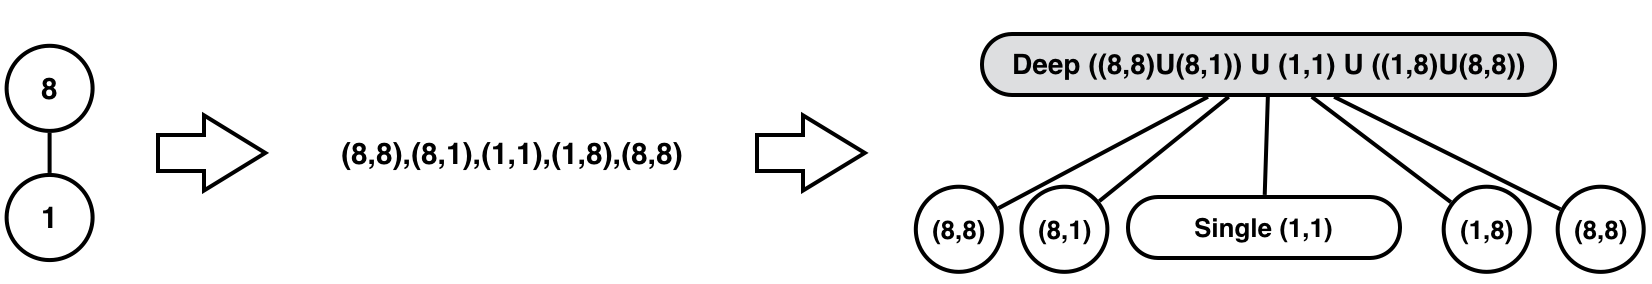
\includegraphics[scale=0.35]{./Images/t1et1ft1} 
\end{center}
\caption{Tree $t_8$ and its corresponding Euler tour $et_8$ and finger tree $ft_8$}
\label{fig:t1et1ft1}
\end{figure}

As an second example, we have $t_2$, Figure~\ref{fig:t2et2ft2}. The spine of the finger tree now contains a \code{Single} type constructor altogether with a \code{Node3}. Again, shadowed ellipses refer to the monoidal annotations \code{Set} where the set-insertion and set-union take place \textit{automatically}.
\begin{figure}
\begin{center}
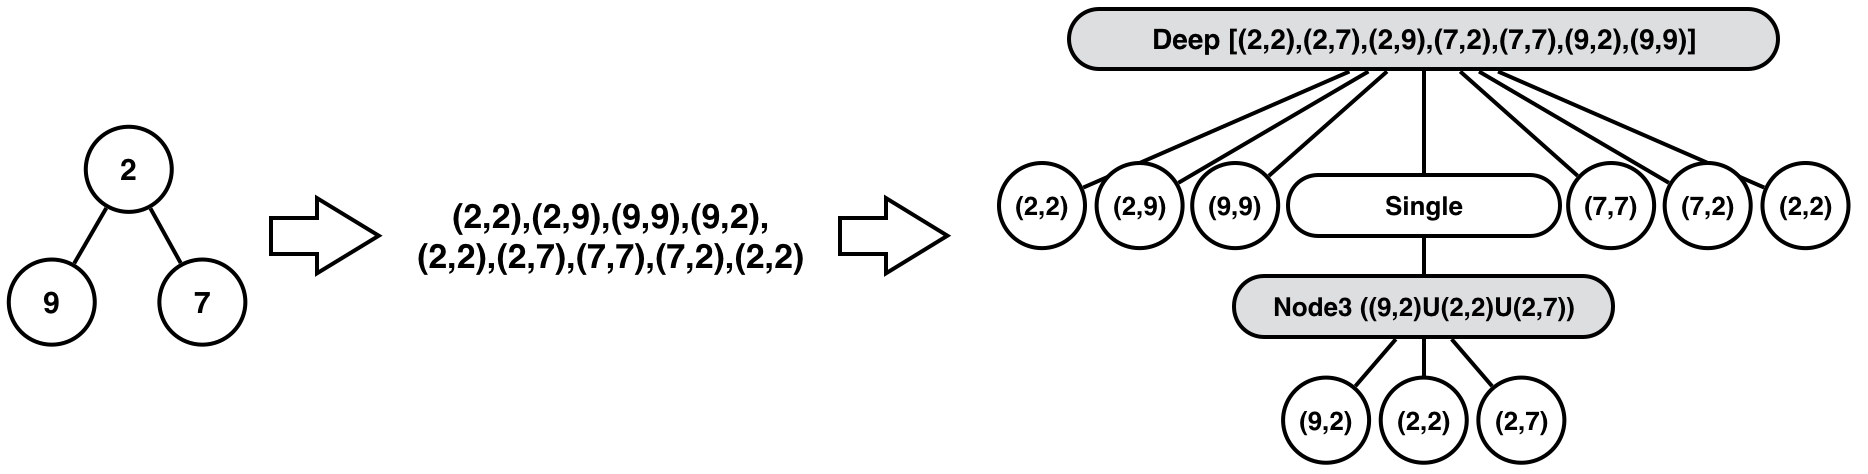
\includegraphics[scale=0.35]{./Images/t2et2ft2} 
\end{center}
\caption{Tree $t_2$ and its corresponding Euler tour $et_2$ and finger tree $ft_2$}
\label{fig:t2et2ft2}
\end{figure}

Now, the forest $f$ in Figure~\ref{fig:forest} is formed by inserting $ft_8$ and $ft_2$ from left and right respectively, in $O(1)$. The forest's \code{Deep} type constructor has the set-union of all the finger trees ($ft_8$ and $ft_2$), depicted in back colour with white font. The thick lines coming out from the top ellipse are the components of the top finger tree: two \code{Digit} and an \code{Empty} subtree (or subforest).
\begin{figure}
\begin{center}
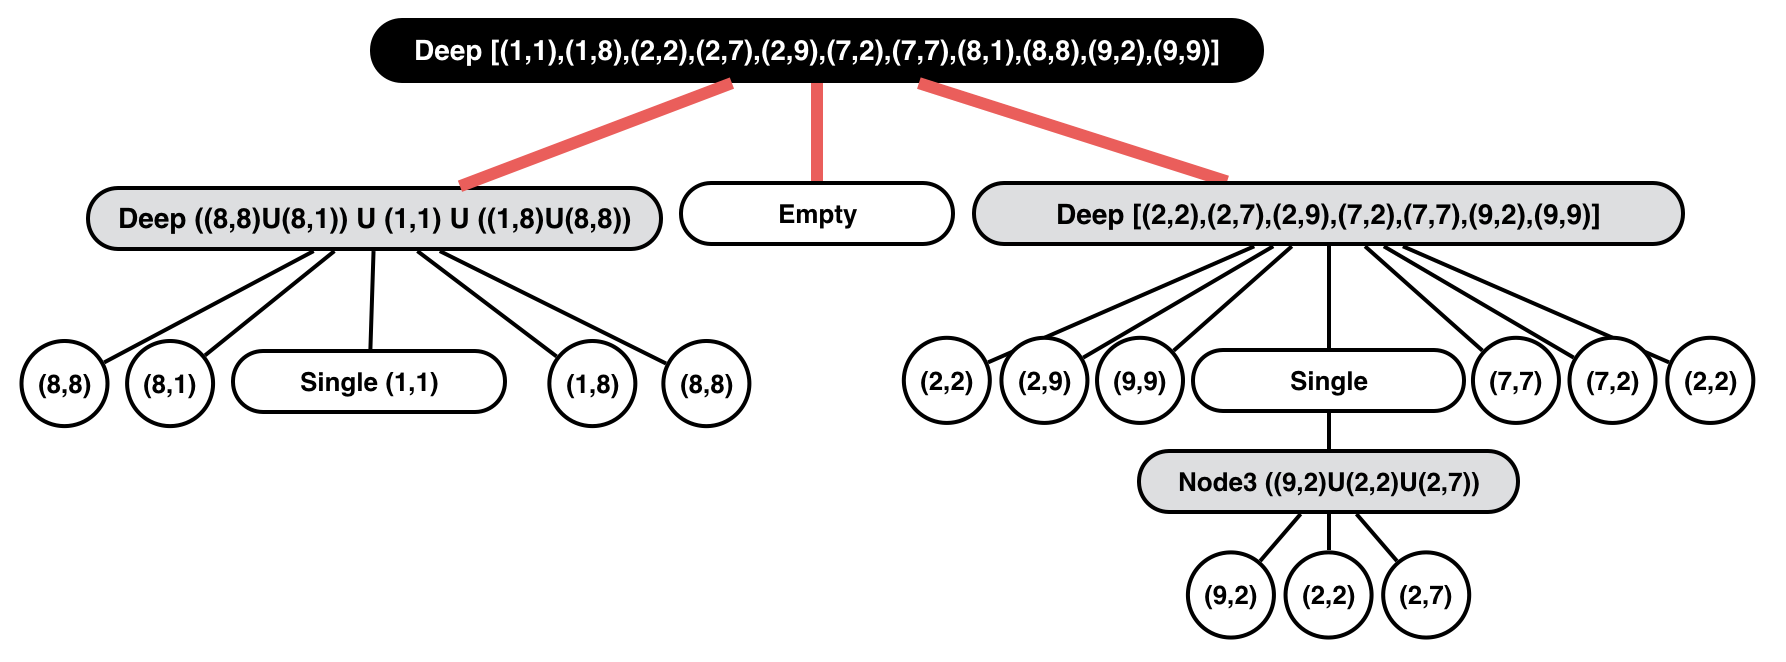
\includegraphics[scale=0.35]{./Images/forest} 
\end{center}
\caption{The forest $f$ comprising finger trees (Euler tours) as elements}
\label{fig:forest}
\end{figure}

Following, we have the basic operations for dynamic trees. Left side of Figure~\ref{fig:rootReroot} shows the \code{root} of a tree $t$ returning a vertex $v$, which is the first element of its finger tree $ft$, implemented in \code{viewl}. Rerooting a tree, by calling \code{reroot}, ask for a vertex $v$ and returns a \textit{new} tree. This is depicted in right side of Figure~\ref{fig:rootReroot}. This operation involves split, concatenation and insertions detailed in Section~\ref{sec:TechDes}.
\begin{figure}
\begin{center}
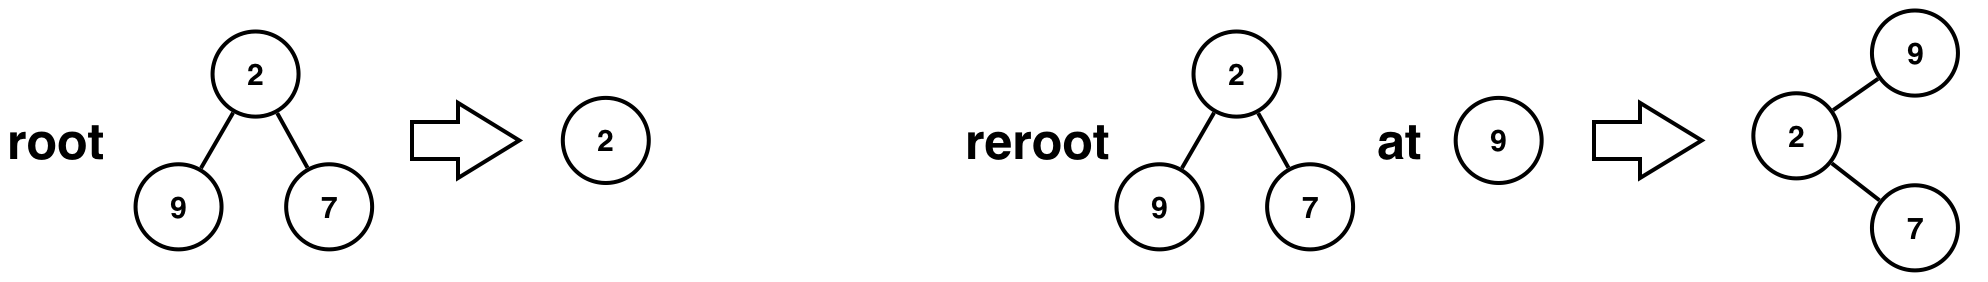
\includegraphics[scale=0.3]{./Images/rootReroot} 
\end{center}
\caption{\textit{root} and \textit{reroot} of a tree}
\label{fig:rootReroot}
\end{figure}

Splitting a finger tree, \code{split}, returns two subtrees (i.e. left and right) and an element, either a pair or an Euler tour, depending on the top container, a tree or a forest. This is depicted in Figure~\ref{fig:split}.
\begin{figure}
\begin{center}
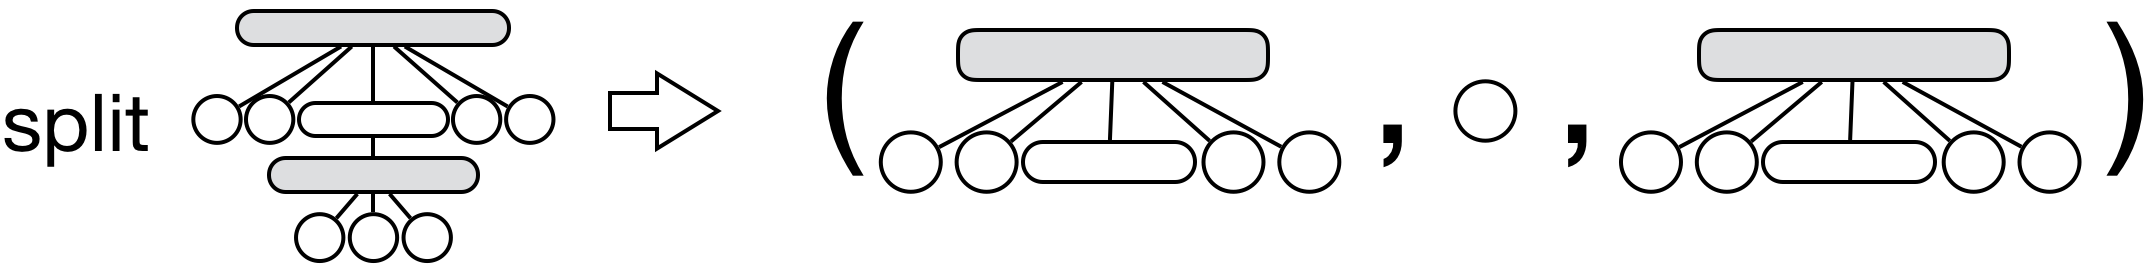
\includegraphics[scale=0.25]{./Images/split} 
\end{center}
\caption{Splitting a tree returns two smaller trees altogether an element}
\label{fig:split}
\end{figure}

Concatenating (also called appending) takes two finger trees and returns another (bigger) finger tree, as in Figure~\ref{fig:concatenation} and its represented by the $\bowtie$ symbol.
\begin{figure}
\begin{center}
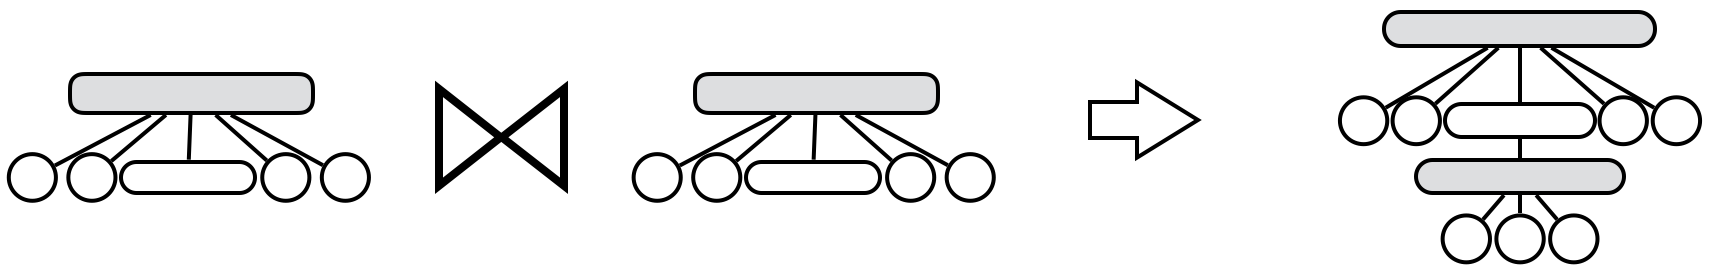
\includegraphics[scale=0.25]{./Images/concatenation} 
\end{center}
\caption{Concatenating two trees, returns a new one bigger}
\label{fig:concatenation}
\end{figure}


\tcr{Since the split operation over finger trees is central to the code, the paper would benefit from a more thorough explanation than the current incomplete type signatures (Concretely I'm missing an explanation of split's two first arguments).}


\tcr{The paper heavily builds on finger trees and tries to explain what they are and how they work, but omit aspects that are crucial to the understanding of the paper. In particular the `split` function is not explained, only listed in Table 2, but used in almost every listing later in the paper. The type listed for `split` mentions an unexplained type constructor `Split` and its type does not match the uses of `split`. The explanation around Fig. 5 does not help. What are the two first arguments to `split`?}




Under Figure~\ref{fig:consleftsnocright} we depict the final four help-functions that support \textit{link} and \textit{cut}: \code{viewl}, $\lhd$ (or \textit{cons}), $\rhd$ (or \textit{snoc}) and \textit{viewr}.
\begin{figure}
\begin{center}
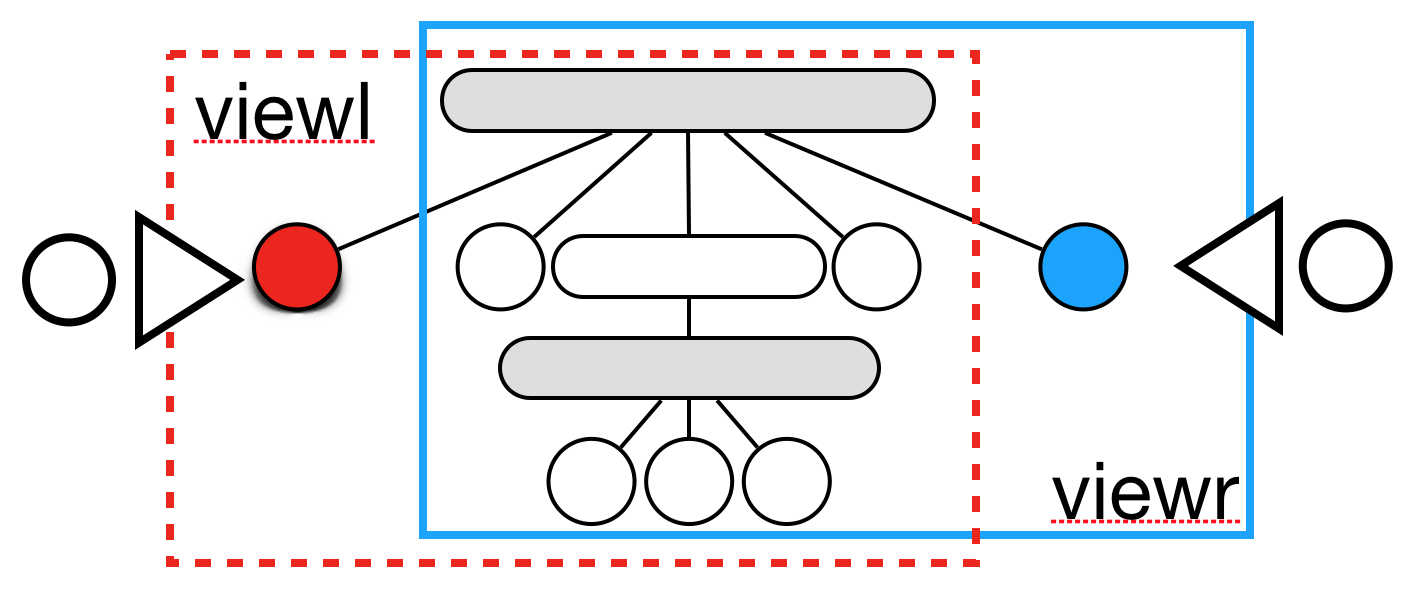
\includegraphics[scale=0.25]{./Images/consleftsnocright} 
\end{center}
\caption{Inserting and viewing from left (\code{viewl},$\lhd$) and inserting and viewing from right (\code{viewr},$\rhd$) }
\label{fig:consleftsnocright}
\end{figure}








\section{dynTsET Design}
\label{sec:TechDes}  


In this section, we present the data types and the operations to manage dynamic trees through Euler-tour trees. Firstly, we describe how to convert any-degree tree into a Euler-tour tree. Secondly, assuming we are provided with Euler-tour trees, we stored them within the leaves of a finger tree. Also, we detail the functions for linking and cutting trees when performed in isolation. Finally, we incorporate the Euler-tour trees into the context of a forest. At this point, we describe the three operations regarded to dynamic trees: \connected, \link and \cut for trees (nodes and edges) within a forest. At any time, the number of nodes is fixed and every node is uniquely identified. Full source code is located at \url{https://github.com/jcsaenzcarrasco/ETdynTs}.


\subsection{From $k$-degree tree to Euler-tour tree}

In Haskell, any-degree tree is also known as multiway tree or rose tree. Actually, there is a library that defines such trees, \code{Data.Tree}, in the Haskell community's central package archive (Hackage).

\begin{lstlisting}
data Tree a = Node {
        rootLabel :: a,         
        subForest :: Forest a   
    }
\end{lstlisting}

So, a tree is a node of type \code{a} (i.e. its root) altogether with a list (possibly empty) of subtrees, seen as forest of type \code{Forest a}. Analogous to multiway trees, our trees (finger trees holding Euler-tours) can not be empty. 

Firstly, we turn a tree into a list of nodes, by attaching (mapping) the prefix and suffix of current node to inner subtrees. We later feed this list into a finger tree. 

\begin{lstlisting}[mathescape] 
rt2et :: (Eq a) $\Rightarrow$ Tree a $\to$ [(a,a)] 
rt2et (Node x ts) = case ts of
  [] $\to$ [(x,x)]
  _  $\to$ root ++ concat ( map ($\lambda$t $\to$ pref t ++ rt2et t ++ suff t) ts )   
    where
     pref v = [(x,rootLabel v)]
     suff v = [(rootLabel v,x)]
     root   = [(x,x)] 
\end{lstlisting} 

Since \code{concat} and \texttt{++} take $O(n)$ where $n$ is the size of the input tree, \code{rt2et} takes $O(n)$. \tcr{Should we need to prove this ???}

The corresponding forest transformation to list of pairs is simply the application of \code{rt2et} to every element in the tree list. Because it requires a single traversal, \code{rt2et} requires $O(n)$ time, where $n$ is the number of elements in the forest.

\begin{lstlisting}[mathescape] 
rf2et :: (Eq a) $\Rightarrow$ Forest a $\to$ [[(a,a)]]
rf2et []          = []
rf2et [Node x []] = [[(x,x)]]  
rf2et (t:ts)      = (rt2et t) : rf2et ts
\end{lstlisting}

Once a tree $t$ of any degree is turned into an Euler tour $et$, we are able to manage $et$ as a sequence. 


\subsection{Euler-tour tree as finger trees of pairs}

Since finger trees work efficiently on sequences, according to \cite{FTs}, we tailored the finger tree in order to support \link, \cut and \connected operations over unrooted trees following the procedures for modifying encodings (i.e. any-degree trees to Euler-tours) by Henzinger and King in \cite{Rand-DynGs-Algos}.

Recall from Figure~\ref{fig:FTdatatype}, the finger tree \code{data FingerTree v a}, has two polymorphic types, the first one (\code{v}) is the type of the monoidal annotation and the second (\code{a}) the type of the values stored at the leaves, which in our case is the sequence type. We have mentioned in the previous section that edges and nodes can be represented as pairs, therefore our values type is \code{(a,a)} for any type \code{a}. In this manner, a pair $(u,v)$ (atomic element in the sequence) represents a node, when $u = v$, and an edge when $u \neq v$. From here, every element in the sequence  can be located.

In the next sections, for practical reasons, we define our pairs of type \code(Int,Int). For the internal finger trees nodes (monoidal annotations), where searching take place, we define \code{Data.Set (a,a)} as our type. By doing so, we are able to take advantage from some set-like operations such as membership-test, insertion and union. 

We define the set-insertion operation every time a pair (either edge or node) is added to an Euler-tour tree (i.e. finger tree). In Haskell, we can see this as
\begin{lstlisting}[mathescape]
import Data.FingerTree
import qualified Data.Set as S

type TreeEF   a = FingerTree (S.Set (a,a)) (a,a)

instance (Ord a) $\Rightarrow$ Measured (S.Set (a,a)) (a,a) where 
   measure (x,y) = S.insert (x,y) S.empty 
\end{lstlisting} 

We shall see in Section~\ref{DoNotKnowYet} that \code{S.Set} can be easily replaced by another set alike data structure as long as this provides membership-testing, insertion, empty-set, set-union and search operations. Also in Section~\ref{sec:Eval} we shall analyse the differences in performance when the monoidal type is changed.

The set-union is already defined in \code{Data.Set} at its monoidal binary operation, therefore there is no need to define this in our proposal.


\subsection{rooting and rerooting a tree}
We shall see later in the definition of \link, \code{link} \cut, and \connected, that functions \root and \reroot are essential. We mentioned earlier that dynamic trees is about managing unrooted trees. By \root we refer to the entry point of any Euler-tour, which always starts in the form $(v,v)$ since it represents a node. By \emph{unrooted} tree we refer to the fact that any node in the tree can be its \root.

Since any-size Euler-tour is represented from now on by a finger tree, we define our initial operation by calling the leftist element as the \root of it, through the function \code{viewl}
\begin{lstlisting}[mathescape] 
root :: Ord a $\Rightarrow$ TreeEF a $\to$ Maybe a  
root tree = case viewl tree of
  EmptyL   $\to$ Nothing
  x :< _   $\to$ Just ( fst x )
\end{lstlisting}

We return the first element in the pair $(v,v)$ since any $v$ represents the node-root. Time complexity of \root is $O(1)$ since \code{viewl} performs $O(1)$ in the finger tree and we simply pattern match over its results.

Then, for \code{reroot}ing a tree we follow partially the second procedure by Henzinger and King in \cite{Rand-DynGs-Algos}, which states:
\begin{displayquote}
\emph{To change the root of \textit{T} from $r$ to $s$}: Let $o_s$ denote any occurrence of $s$. Splice out the first part of the sequence ending with the occurrence before $o_s$, remove its first occurrence ($o_r$), and tack the first part on to the end of the sequence, which now begins with $o_s$. Add a new occurrence $o_s$ to the end.
\end{displayquote}

So, instead of looking for $r$ (old root) occurrences, we focus only in the new root($s$). We splice out the first and second occurrences of node $s$ by simply searching for it as $(s,s)$ in the finger tree. Then, simply glue all the parts in order, that is, the new root first (leftist) followed by the second and first occurrences of $s$. This is denoted in the following snippet.

\begin{lstlisting}[mathescape]
reroot :: Ord a $\Rightarrow$ TreeEF a $\to$ a $\to$ TreeEF a 
reroot tree node = case (FT.search pred tree) of
   Position left _ right $\to$ rootTree $\lhd$ (right $\bowtie$ left)
   _                     $\to$ tree
 where rootTree      = (node,node)
       pred before _ = (S.member rootTree) before
\end{lstlisting} 

\tcr{PERFORMANCE of REROOT }\tcb{Operators $\lhd$, $\bowtie$ and \code{FT.search} take $O(\log n)$ amortised on finger trees. Since we are applying them only once, our \code{reroot} function also takes $O(\log n)$}. In case \code{reroot} is asked altogether with a node not in the tree, it simply returns the original \code{tree}.

The following two functions, \code{linkTree} and \code{cutTree} are regarded to trees off a forest. Again, following Henzinger and King, first procedure in \cite{Rand-DynGs-Algos}:
\begin{displayquote}
\emph{To delete edge \{$a$,$b$\} from $T$:} Let $T_1$ and $T_2$ be the two trees that result, where $a \in$ $T_1$ and $b \in$ $T_2$. Let $o_{a_1}$, $o_{b_1}$, $o_{b_2}$ represent the occurrences encountered in the two traversals of \{$a,b$\}. If $o_{a_1} < o_{b_1}$ and $o_{b_1} < o_{b_2}$, then $o_{a_1} < o_{b_1} < o_{b_2} < o_{a_2}$. Thus, ET($T_2$) is given by the interval of ET($T$) $o_{b_1}$, \ldots, $o_{b_2}$ and ET($T_1$) is given by splicing out of ET($T$) the sequence $o_{b_1}$, \ldots, $o_{a_2}$. 
\end{displayquote} 

Deleting an edge means \emph{cut}ting a tree through such edge. The following snippet shows the \code{cutTree} operation analogous to the above procedure :
\begin{lstlisting}[mathescape]
cutTree :: Ord a $\Rightarrow$ a $\to$ a $\to$ TreeEF a $\to$ Maybe (TreeEF a,TreeEF a) 
cutTree u v tree = case FT.search predUV tree of
 Position left _ right $\to$
   case (FT.search predVU left ) of
      Position leftL _ rightL $\to$  
        Just (rightL, leftL $\bowtie$ right)
      _                $\to$                    
        case (FT.search predVU right) of
          Position leftR _ rightR $\to$
            Just (leftR, left $\bowtie$ rightR)
          _ $\to$ Nothing 
 _  $\to$ Nothing  
 where
   predUV before _ = (S.member (u,v)) before 
   predVU before _ = (S.member (v,u)) before 
\end{lstlisting}

The snippet quite follows the procedure. The pairs $(u,v)$ and $(v,u)$ are left out the resulting sequences in the wildcards in lines 3, 5 and 9. Since we search $(u,v)$ first, there are only two possibilities for $(v,u)$ to be part of. If it is on the left we build up $T_1$ from \code{rightL}, and $T_2$ from \code{leftL} and \code{right}. Otherwise $T_1$ is built from \code{leftR} and $T_2$ from \code{left} and \code{rightR}.

\tcr{PERFORMANCE of CUT }\tcb{Operator $\bowtie$ and function \code{FT.search} take $O(\log n)$ amortised on finger trees. Since we are applying them twice, our \code{cut} function also takes $O(\log n)$}. In case \code{cut} is called with with nodes belonging different components or the edge in matters in not found, then \code{cut} returns \code{Nothing}, which will be captured as failure in \cut within a forest operation.


 

\section{Experimental Evaluation} 
\label{sec:Eval} 


This section presents experiments to evaluate how much running time costs in terms of performance. The experiments will show that, in practice, \dyntset is faster by a factor of $O(\log n)$ per operation than that of the theoretical analysis (Section\ref{sec:TechDes}).

This section is organised as follows. Firstly, we describe the experimental setup. Secondly, a brief description in the implementation of test sets is provided. We then present experimental studies of the three different operations in \dyntset. Finally, we present an additional experiment for the cases where laziness as speeding up factor in favor of the running times for the dynamic tree operations.


\subsection{Experimental Setup}
Functions \link, \cut, \conn, \code{root} and \code{reroot} were implemented by the author in Haskell and compiled with \code{ghc} version 8.0.1 with optimisation \code{-O2}. The experiments were performed on a 2.2 GHz Intel Core i7 MacBook Pro with 16 GB 1600 MHz DDR3 running macOS High Sierra version 10.13.1 (17B1003). We imported the following libraries into our code from the online package repository Hackage: \cite{HaskellFT} code for finger trees, \cite{HaskellSet} for conventional sets and \cite{HaskellEdison} for lazy sets.

The running time of a given computation was determined by the mean of three executions.

\subsection{Data structure} 

The values maintained by the data structures (sets and finger trees) are stored as fixed-precision \code{Int} types, holding values from $-2^{29}$ up to $2^{28}$ although we test only the positive values.

The structures are initialized with a fixed number of nodes (or vertices) $n$; this number does not change during the execution. This allow us to know the initial size of the forest and we subtract it from the benchmarking.

Since \dyntset is not called by any application, the random generation of nodes for \link or \cut does not necessarily be effective. Actually, around 70\% of the generated nodes $x$ and $y$ passed to \link and \cut were not valid, that is, their result turned out to be the original forest. In order to overcome this, we stored the random generated nodes that were effective into a plain files and from there benchmarking the dynamic tree operations.


\subsection{Incremental operations} 
We start with an empty forest (just singleton-trees); given $n=20,000$ nodes we perform $1 \ldots 20,000$ \link operations. Upon reaching a target length, we plot the total time taken. Then, we divide the time taken by the number of operations to calculate the time per operation and then multiply it by a constant (x1000) to make the curve visible in the same chart.

\begin{figure}[H]
\begin{center}
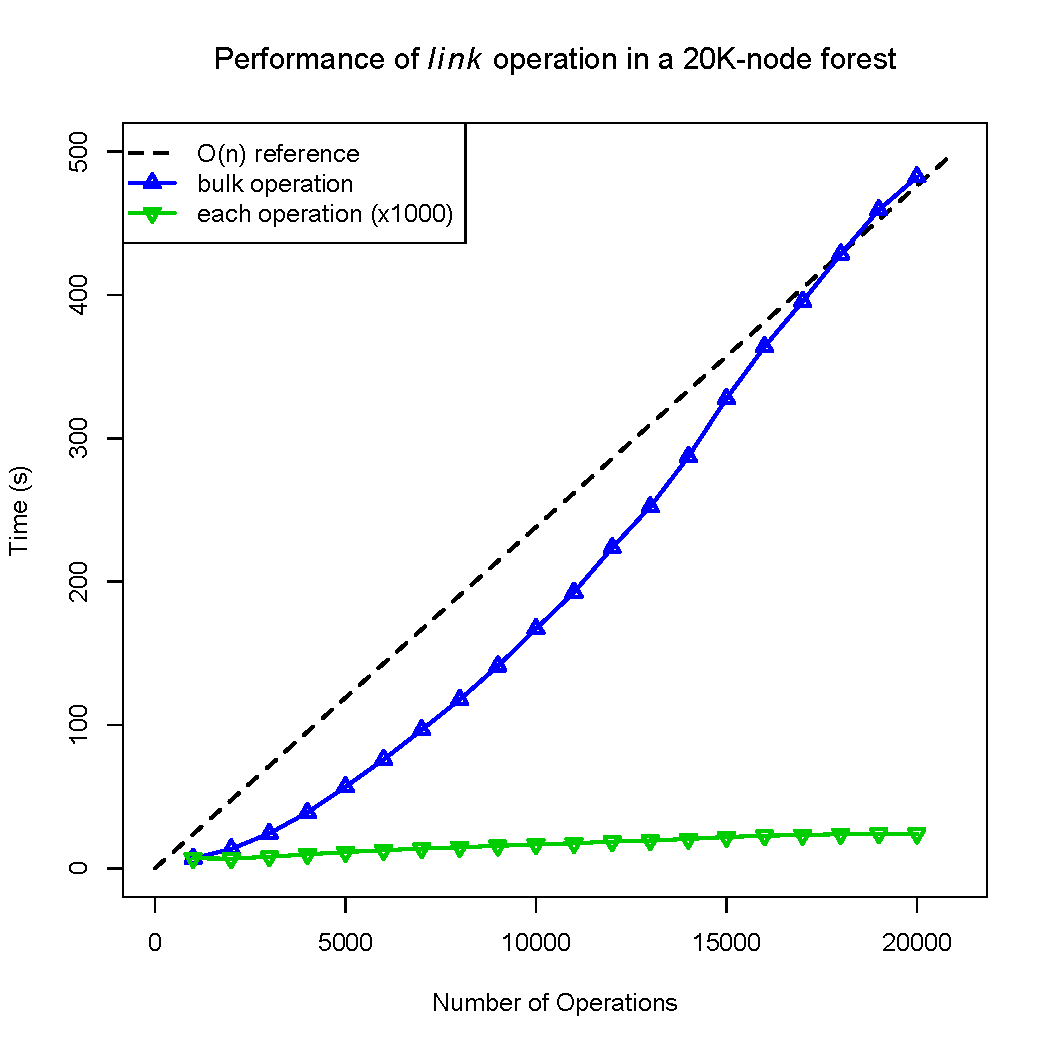
\includegraphics[scale=0.4]{./Images/plotLink} 
\end{center}
\caption{Sequence of {\link}s from empty forest up to a single tree in such forest}
\label{fig:incLink}
\end{figure}

\textit{\emph{Results}}. The behaviour of the curve regarding the time per \link operation shows that in practice it takes $O(1)$ against $O(\log n^2)$ in theory back in Section~\ref{sec:TechDes}, or the linear behaviour by the \link operations in bulk.

\subsection{Fully dynamic operations} 
We start with the incremental process as before for $n=10,000$. Then, for \cut we start in the opposite direction, that is, cutting from a single tree in the forest until only singleton-trees remain in such forest. To this performance we subtract the time take for the incremental bit. For \conn performance we compute first an interleaved operation of \link and \cut (not necessarily in this order). We measure the time taken for \conn followed by the corresponding \link or \cut and then we subtract the interleaved process. The following figures show our three dynamic operations in bulk and per operation.

\begin{figure}[H]
\centering
\begin{subfigure}{.5\textwidth}
  \centering
  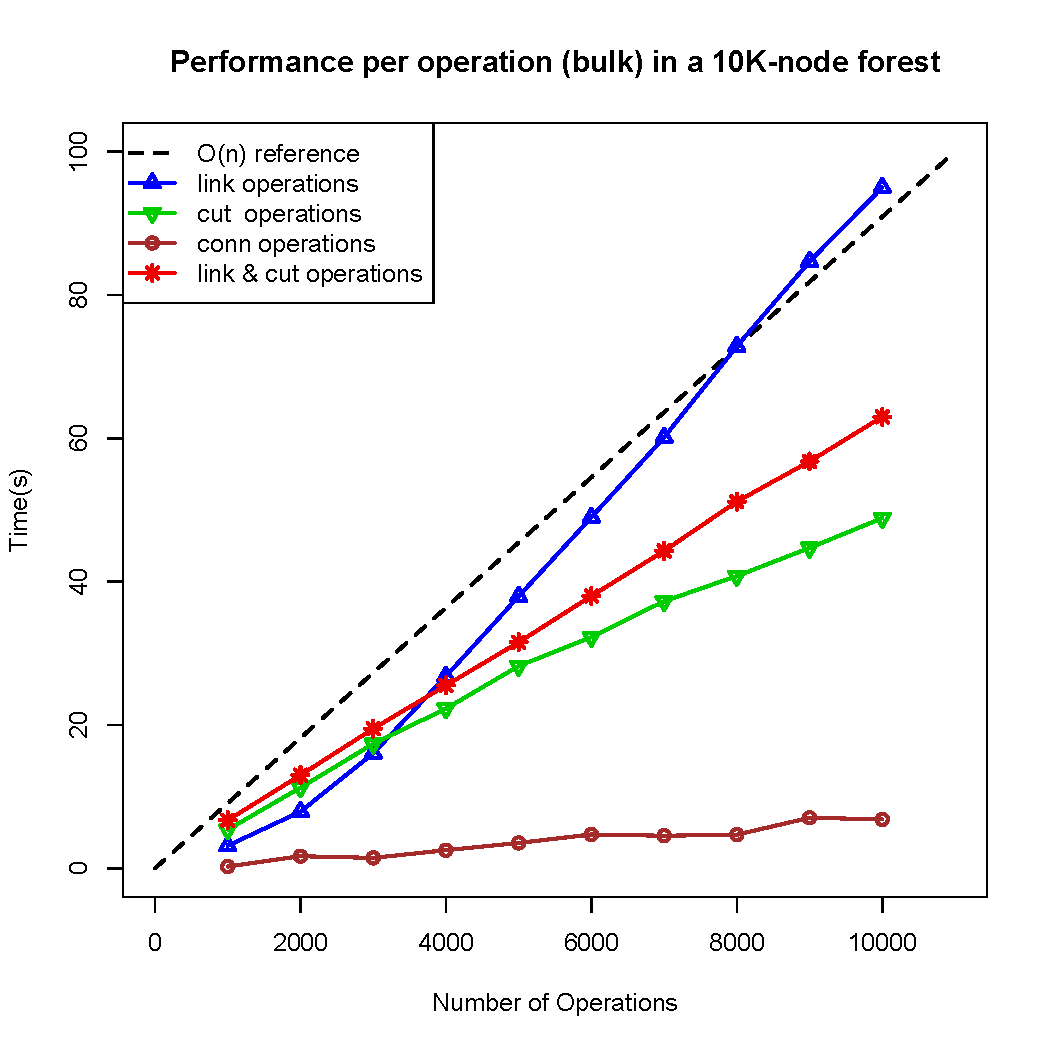
\includegraphics[scale=0.38]{./Images/plotEach}
  \caption{In bulk}
%  \label{fig:sub1}
\end{subfigure}%
\begin{subfigure}{.5\textwidth}
  \centering
  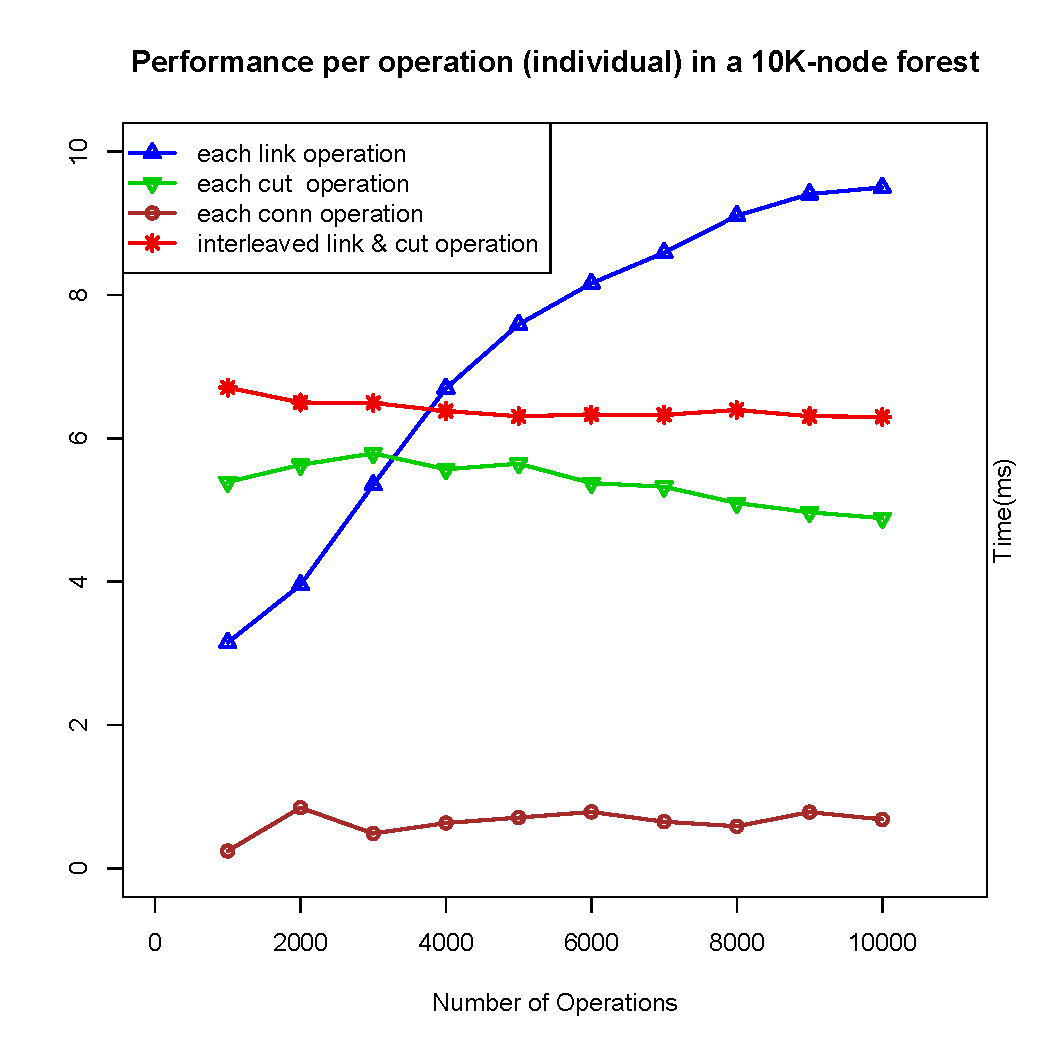
\includegraphics[scale=0.38]{./Images/plotOpsIndiv}
  \caption{Per operation}
%  \label{fig:sub2}
\end{subfigure}
\caption{Time taken by operation, and interleaved \link and \cut}
\label{fig:EachOp}
\end{figure}

\textit{\emph{Results}}. We observe that \cut and \conn obey the same pattern as \link. That is, $O(1)$ time per operation being \textit{connectivity} the fastest of the dynamic tree operations, as expected.

From the above analyses, we notice that \link performs better when is interleaved with \cut. To see this behaviour closer, we present the bulk and individual cases in the following charts varying the forest size under the same amount of operations.

\begin{figure}[H]
\centering
\begin{subfigure}{.5\textwidth}
  \centering
  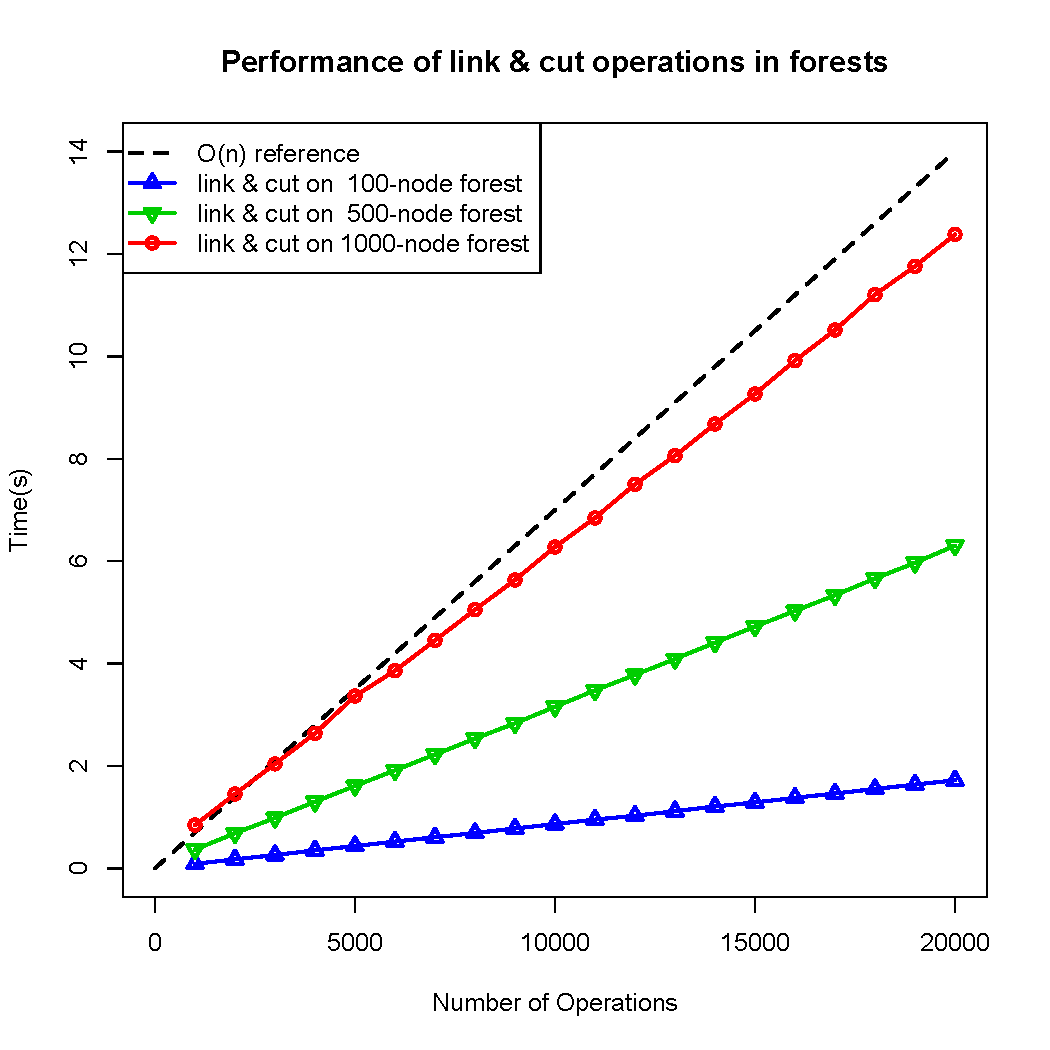
\includegraphics[scale=0.38]{./Images/plotForests}
  \caption{In bulk}
%  \label{fig:sub1}
\end{subfigure}%
\begin{subfigure}{.5\textwidth}
  \centering
  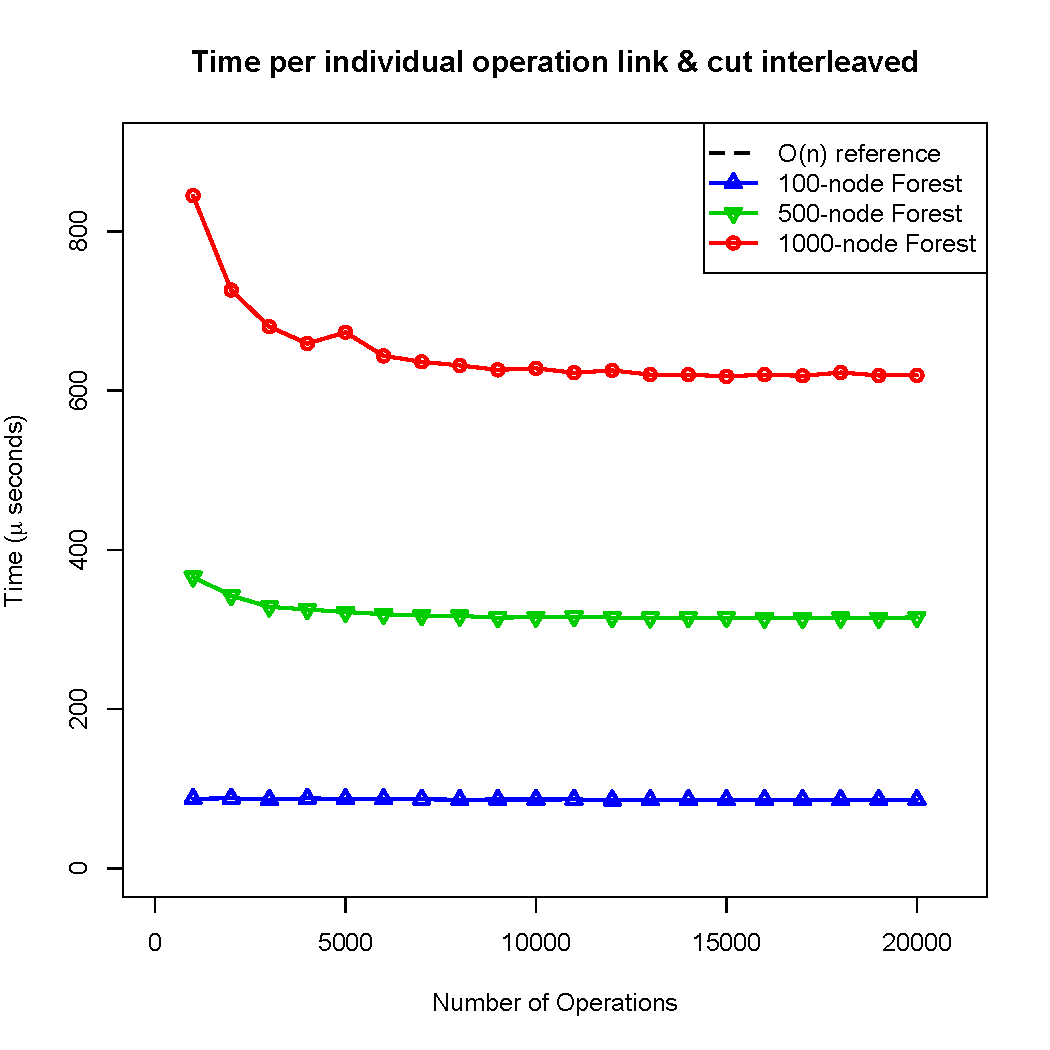
\includegraphics[scale=0.38]{./Images/plotLCForests}
  \caption{Per operation}
%  \label{fig:sub2}
\end{subfigure}
\caption{Time taken when \link and \cut are interleaved with different forest sizes}
\label{fig:EachOp}
\end{figure}

\subsection{Selection of the set data structure}
The set-like data structure is crucial in our implementation and testing of \dyntset since is the search engine for the nodes when any operation is applied to a forest. There are plenty of implementations for such set-like structure, mostly as binary balanced search trees. In our case, where Haskell is a lazy-evaluation language by default, we select two main choices to compare: \code{Data.Set} which is a strict data type definition and \code{Data.Edison.Coll.LazyPairingHeap} which is semi-lazy or semi-strict data type. The following figure shows the performance for each.

\begin{figure}[H]
\begin{center}
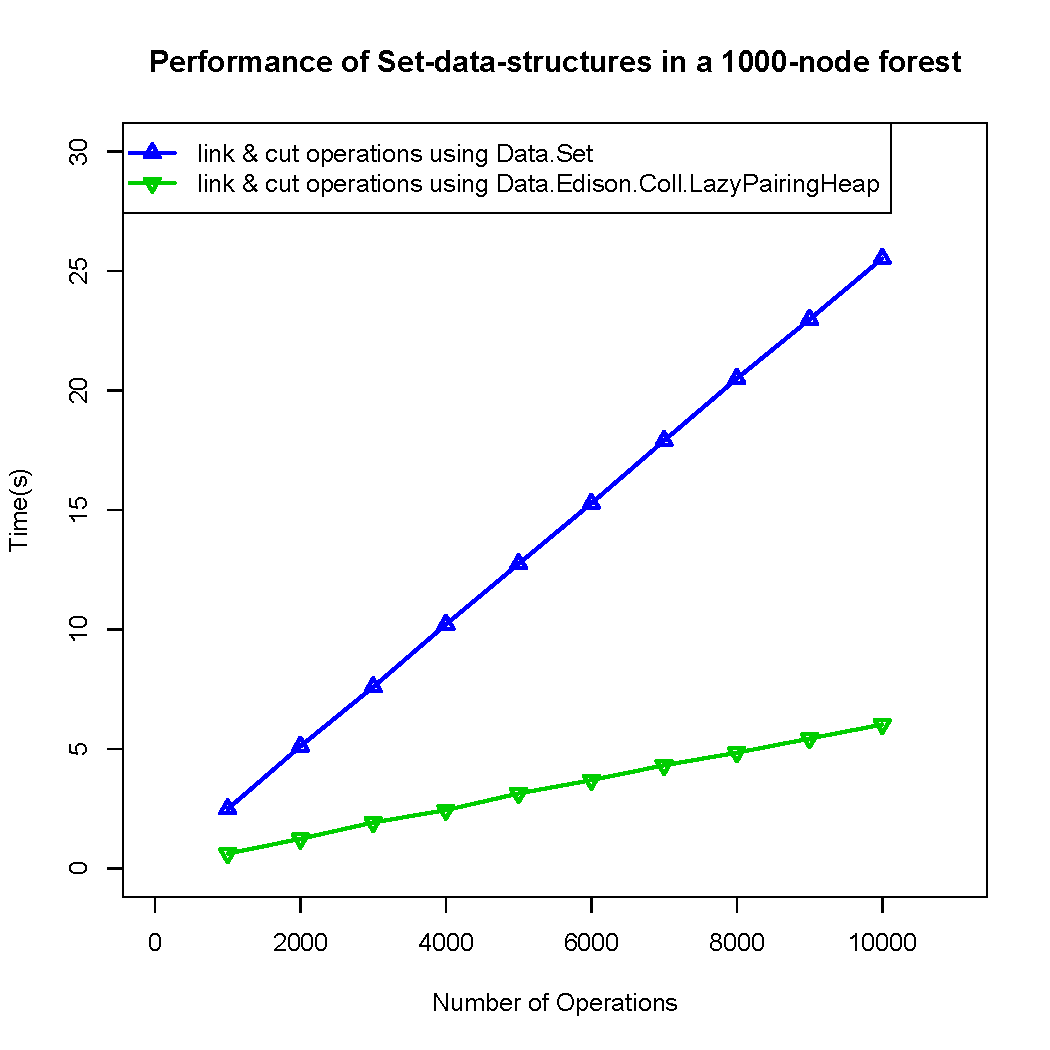
\includegraphics[scale=0.4]{./Images/plotSets} 
\end{center}
\caption{Dynamic operations through different sets structures as monoidal annotations}
\label{fig:plotSets}
\end{figure}

The above curves show that, although by a constant factor, laziness speeds up the running time in the computation of dynamic tree operations through the set-like data structures.

\tcb{Amortised over what??}
 

\section{Related Work} 
\label{sec:RelWrk} 

Approaches different to our own have, of course, been taken by other researchers, in particular by Dexter et al. \cite{Lazy-Gproc-Haskell} as well as by Headley and Hammer \cite{RAZ}. The former uses techniques to delay the computation of updates and the latter uses lighter and simpler data structures. Considering our own work alongside these approaches leads us to suggest that it may be possible to produce an interesting combination of the three, since there are at least three aspects we have found to be experimentally time-consuming in practice:

\begin{enumerate}
\item an Euler tour is treated as a sequence by efficient structures like finger trees, but the corresponding tree-like operations are also involved in update operations. A mixed, or lighter structure is an essential step towards achieving general efficiency;

\item the unbounded sequence of update operations results in a need to maintain the whole structure. In this context persistence triggers the consumption of memory allocation, and this suggests that benefits may accrue if we were to use higher order programming with effects;

\item the internal nodes of our finger tree structure hold the internal monoid \code{Set}, which is the most time-consuming element in our code and experimental results. Since rebalancing is an essential property of the internal binary search tree in \code{Set}, we propose conducting an analysis and design of different new balanced binary search tree as monoid in future work.
\end{enumerate}
 

\section{Conclusion and Future Work} 
\label{sec:Concl} 

Although we have presented evidence that ETFT trees are efficient data structures for dynamic tree handling, we have noticed experimentally that there is plenty of work to do specifically in the stream of interleaved operations applied as input to the data structure, that is, the unbounded sequence of updates and queries.

Finally, there is an evident need for a library of well-crafted test cases against which implementations of dynamic trees and graphs can be tested. At present, for example, there is little to guide us when generating the update-sequences against which our structures are validated, and this raises a number of obvious issues. For example,

\begin{itemize}
\item Can we find test sets which guarantee coverage of key properties?

\item Which properties are we interested in?

\item If we know the general ratio of updates to queries (say), can we identify a more specific data structure to enhance efficiency still further?

\item Or maybe it’s enough to test solutions empirically, using live data from (say) the ever-changing structure of links in the Internet of Things?

\end{itemize}

These and other questions remain to be addressed, but we believe the quest for efficient dynamic data structures will become ever more important as seek to model, simplify and reason about the increasingly dynamic algorithmic structures in which modern culture is immersed and on which it depends.


\tcb{Uniqueness on edges allow to carry labels, therefore ETFT could be the core for other approaches to dynamic trees such link-cut trees. Examples, illustrations, references ?? } 

\tcb{Acknowledgements:  chahine.moreau@gmail.com ?? } 

\bibliography{./Refs/refs}

%\begin{thebibliography}{4}
%\input{./Refs/refs.bib}
%\end{thebibliography} 

\end{document}
